\documentclass[RT]{UTNLSE}
\usepackage{comment}
\usepackage{graphicx}
\usepackage{siunitx}
\usepackage{tabularray}
\usepackage{geometry}
\usepackage{amsmath}
\usepackage{float}
\usepackage{listings}
\usepackage{xcolor}
\usepackage{hyperref}
\usepackage{booktabs}
\usepackage{array}
\usepackage{enumitem}
\usepackage{multirow}
\usepackage{tikz}
\usetikzlibrary{positioning, shapes.geometric, arrows.meta, fit, backgrounds, calc, babel, decorations.pathreplacing}

\titleES{Resolución de la Parte Teórica: Modo Protegido}
\addauthor{Fuster}{Lucio}{UTN, FRA, Avellaneda, Buenos Aires, Argentina}{N/A}

\resumenES{Resolución del cuestionario teórico correspondiente a la Evaluación Globalizadora B, abordando los mecanismos de protección de memoria del 80x386, descriptores, el Segmento de Estado de Tarea (TSS) y el proceso de paginado.}
\keywordsES{Modo Protegido; 80x386; GDT; LDT; TSS; Paginado; UTN FRA}

\begin{document}

% ============================================================
\section{Mecanismos de Protección de acceso al Segmento en Modo Protegido}
% ============================================================

\subsection*{a. Diagrama del mecanismo de protección de memoria del 80x386}
En Modo Protegido, el procesador no accede directamente a la dirección física a través de los registros de segmento. En su lugar, el valor cargado en un registro de segmento (CS, DS, SS, ES, FS, GS) se denomina \textbf{Selector}. Este selector ya no contiene la dirección base, sino un índice que apunta a una tabla de descriptores ubicada en memoria RAM. Es el \textbf{descriptor} (y no el programa) el que contiene la base, el límite y los atributos de protección del segmento; por eso el programa no puede acceder directamente al segmento: siempre debe pasar por la verificación del procesador.

La Figura~\ref{fig:overview} muestra la visión general de la traducción de direcciones, la Figura~\ref{fig:lookup} detalla cómo el selector localiza el descriptor y la Figura~\ref{fig:checks} las verificaciones de protección que se hacen antes de generar la dirección lineal.

\begin{figure}[H]
\centering
\resizebox{\textwidth}{!}{%
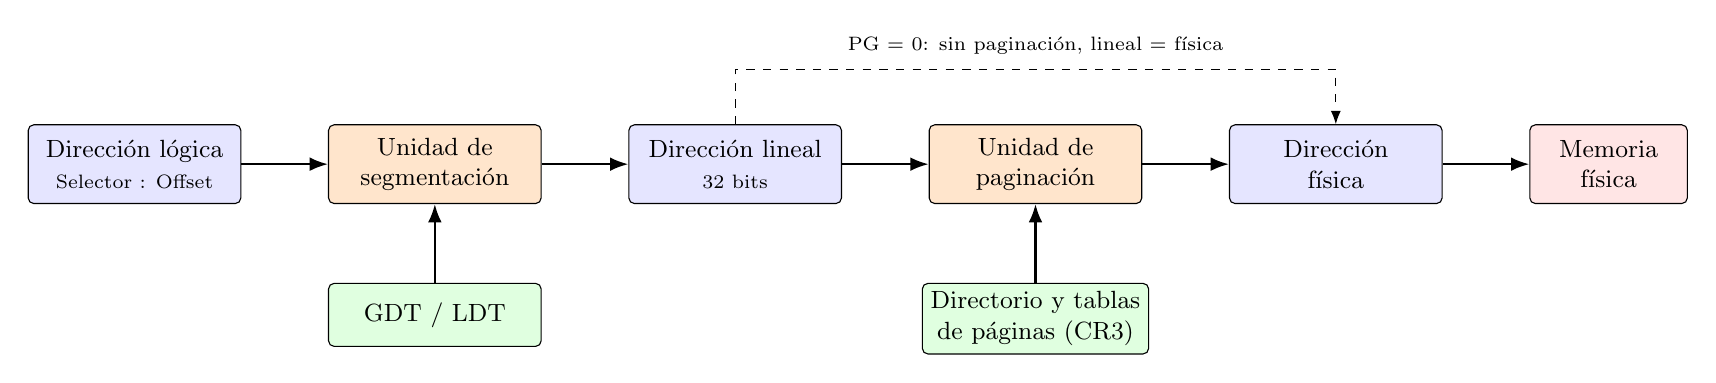
\begin{tikzpicture}[font=\small,
    blk/.style={draw, rounded corners=2pt, align=center, minimum height=10mm, minimum width=27mm, inner sep=3pt},
    addr/.style={blk, fill=blue!10},
    unit/.style={blk, fill=orange!20},
    tbl/.style={blk, fill=green!12, minimum height=8mm}]
    \shorthandoff{<>}
    \node[addr] (log) {Dirección lógica\\ {\scriptsize Selector : Offset}};
    \node[unit, right=11mm of log] (seg) {Unidad de\\segmentación};
    \node[addr, right=11mm of seg] (lin) {Dirección lineal\\ {\scriptsize 32 bits}};
    \node[unit, right=11mm of lin] (pag) {Unidad de\\paginación};
    \node[addr, right=11mm of pag] (phy) {Dirección\\física};
    \node[blk, fill=red!10, right=11mm of phy, minimum width=20mm] (mem) {Memoria\\física};
    \node[tbl, below=10mm of seg] (dt) {GDT / LDT};
    \node[tbl, below=10mm of pag] (pt) {Directorio y tablas\\de páginas (CR3)};

    \draw[-{Latex}, thick] (log) -- (seg);
    \draw[-{Latex}, thick] (seg) -- (lin);
    \draw[-{Latex}, thick] (lin) -- (pag);
    \draw[-{Latex}, thick] (pag) -- (phy);
    \draw[-{Latex}, thick] (phy) -- (mem);
    \draw[-{Latex}, thick] (dt) -- (seg);
    \draw[-{Latex}, thick] (pt) -- (pag);
    % bypass si PG = 0
    \draw[-{Latex}, dashed] (lin.north) -- ++(0,7mm) -| (phy.north);
    \node[font=\scriptsize] at ($(pag.north)+(0,10mm)$) {PG = 0: sin paginación, lineal = física};
\end{tikzpicture}}
\caption{Traducción de dirección lógica a física en el 80x386.}
\label{fig:overview}
\end{figure}

\begin{figure}[H]
\centering
\resizebox{\textwidth}{!}{%
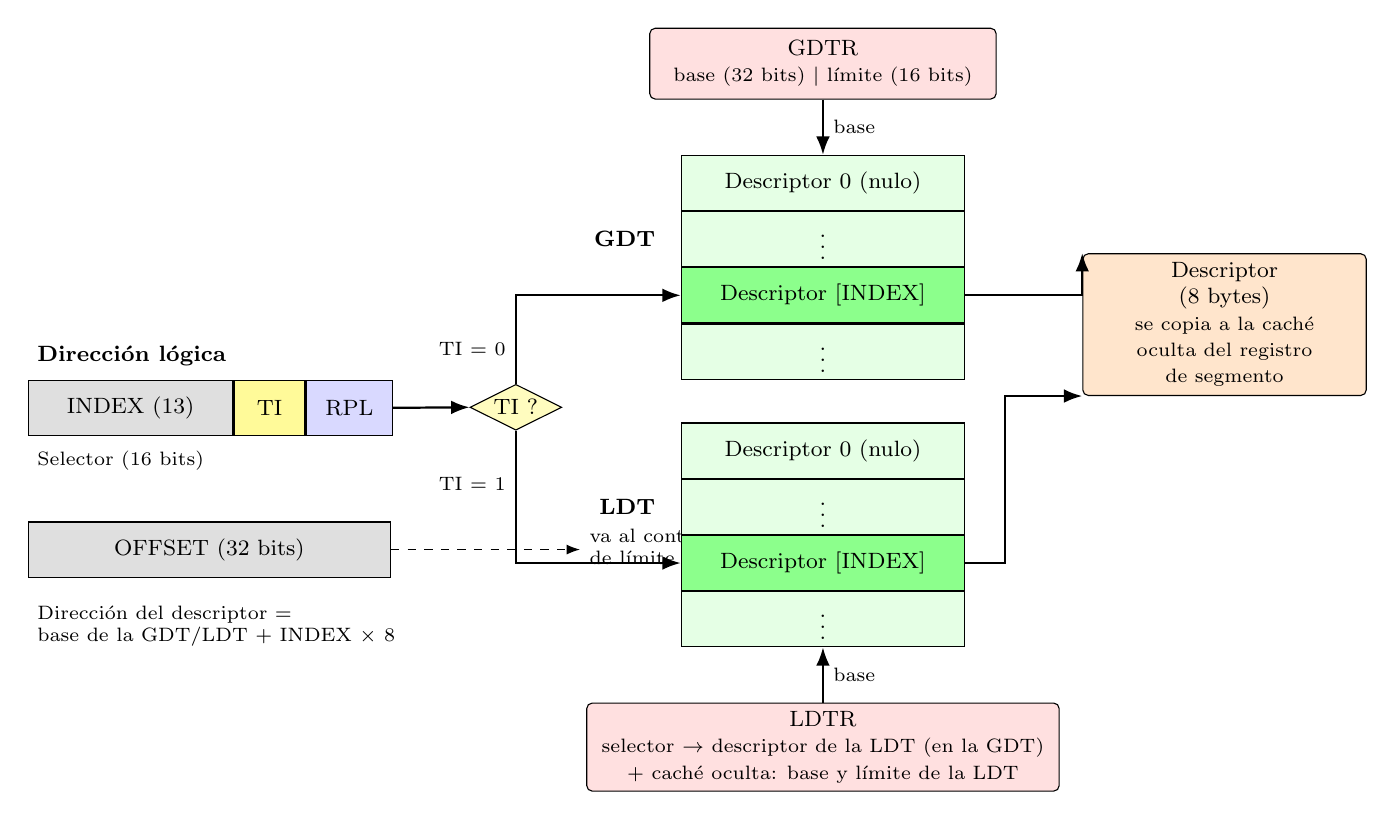
\begin{tikzpicture}[font=\footnotesize,
    blk/.style={draw, align=center, minimum height=7mm, inner sep=2pt},
    row/.style={blk, minimum width=36mm, fill=green!10},
    hit/.style={blk, minimum width=36mm, fill=green!45},
    reg/.style={draw, rounded corners=2pt, align=center, fill=red!12, minimum height=9mm, inner sep=3pt}]
    \shorthandoff{<>}
    % Dirección lógica
    \node[anchor=south west, font=\footnotesize\bfseries] at (0,2.45) {Dirección lógica};
    \node[blk, fill=gray!25, minimum width=26mm, anchor=north west] (idx) at (0,2.4) {INDEX (13)};
    \node[blk, fill=yellow!40, minimum width=9mm, anchor=west] (ti) at (idx.east) {TI};
    \node[blk, fill=blue!15, minimum width=11mm, anchor=west] (rpl) at (ti.east) {RPL};
    \node[anchor=north west, font=\scriptsize] at (0,1.62) {Selector (16 bits)};
    \node[blk, fill=gray!25, minimum width=46mm, anchor=north west] (off) at (0,0.6) {OFFSET (32 bits)};
    \draw[-{Latex}, dashed] (off.east) -- ++(2.4,0) node[right, font=\scriptsize, align=left] {va al control\\de límite (Fig.~\ref{fig:checks})};
    \node[anchor=north west, font=\scriptsize, align=left] at (0,-0.35) {Dirección del descriptor =\\base de la GDT/LDT + INDEX $\times$ 8};

    % Selector de tabla
    \node[diamond, draw, aspect=2, fill=yellow!25, inner sep=1pt] (sw) at (6.2,2.05) {TI ?};
    \draw[-{Latex}, thick] (rpl.east) -- (sw.west);

    % GDT
    \node[row] (g1) at (10.1,4.9) {Descriptor 0 (nulo)};
    \node[row, below=0pt of g1] (g2) {$\vdots$};
    \node[hit, below=0pt of g2] (g3) {Descriptor [INDEX]};
    \node[row, below=0pt of g3] (g4) {$\vdots$};
    \node[left=2mm of g2, font=\footnotesize\bfseries] {GDT};
    \node[reg, above=7mm of g1, minimum width=44mm] (gdtr) {GDTR\\ {\scriptsize base (32 bits) $|$ límite (16 bits)}};
    \draw[-{Latex}, thick] (gdtr.south) -- (g1.north) node[midway, right, font=\scriptsize] {base};

    % LDT
    \node[row] (l1) at (10.1,1.5) {Descriptor 0 (nulo)};
    \node[row, below=0pt of l1] (l2) {$\vdots$};
    \node[hit, below=0pt of l2] (l3) {Descriptor [INDEX]};
    \node[row, below=0pt of l3] (l4) {$\vdots$};
    \node[left=2mm of l2, font=\footnotesize\bfseries] {LDT};
    \node[reg, below=7mm of l4, minimum width=60mm] (ldtr) {LDTR\\ {\scriptsize selector $\rightarrow$ descriptor de la LDT (en la GDT)}\\ {\scriptsize + caché oculta: base y límite de la LDT}};
    \draw[-{Latex}, thick] (ldtr.north) -- (l4.south) node[midway, right, font=\scriptsize] {base};

    % flechas desde TI
    \draw[-{Latex}, thick] (sw.north) |- (g3.west) node[pos=.2, left, font=\scriptsize] {TI = 0};
    \draw[-{Latex}, thick] (sw.south) |- (l3.west) node[pos=.2, left, font=\scriptsize] {TI = 1};

    % caché del descriptor
    \node[draw, rounded corners=2pt, fill=orange!20, align=center, minimum height=18mm, minimum width=36mm, inner sep=3pt] (cache) at (15.2,3.1) {Descriptor\\(8 bytes)\\{\scriptsize se copia a la caché}\\{\scriptsize oculta del registro}\\{\scriptsize de segmento}};
    \draw[-{Latex}, thick] (g3.east) -- (cache.north west |- g3.east) -- (cache.north west);
    \draw[-{Latex}, thick] (l3.east) -- ++(0.5,0) |- (cache.south west);
\end{tikzpicture}}
\caption{Localización del descriptor a partir del selector (bit TI).}
\label{fig:lookup}
\end{figure}

\begin{figure}[H]
\centering
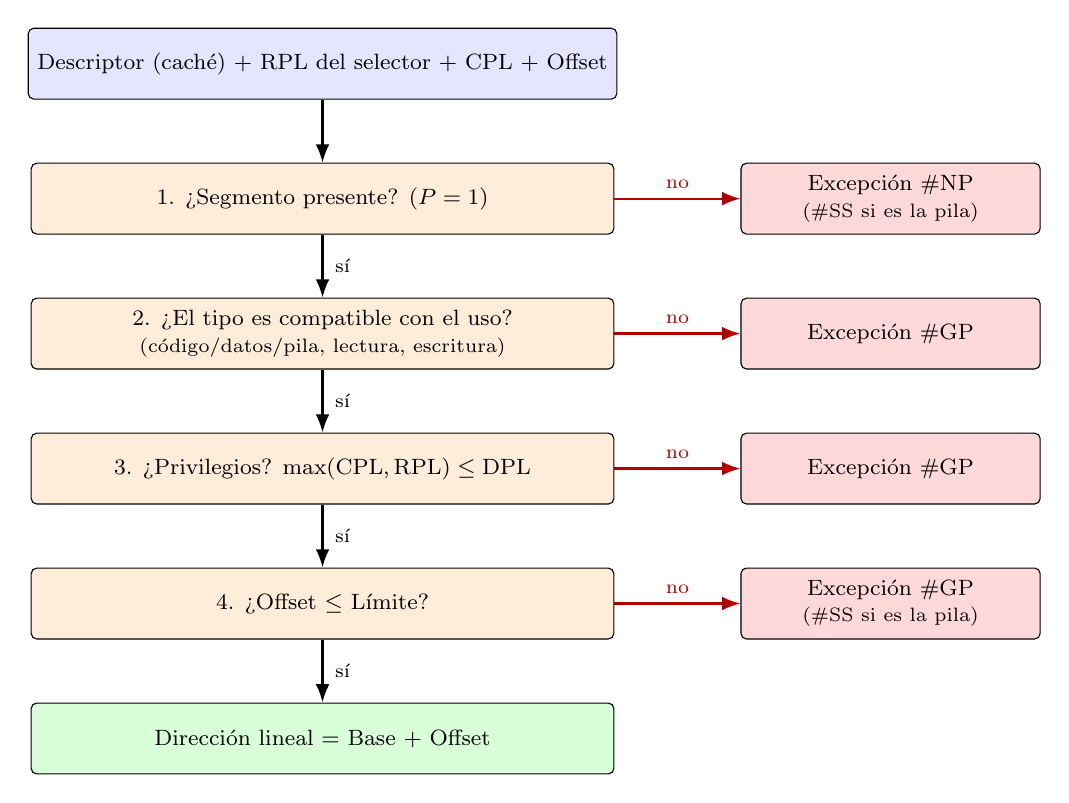
\begin{tikzpicture}[font=\footnotesize,
    chk/.style={draw, fill=orange!15, align=center, minimum width=74mm, minimum height=9mm, rounded corners=2pt},
    exc/.style={draw, fill=red!15, align=center, minimum width=38mm, minimum height=9mm, rounded corners=2pt},
    io/.style={draw, fill=blue!10, align=center, minimum width=74mm, minimum height=9mm, rounded corners=2pt}]
    \shorthandoff{<>}
    \node[io] (in) {Descriptor (caché) + RPL del selector + CPL + Offset};
    \node[chk, below=8mm of in] (c1) {1. ¿Segmento presente? ($P = 1$)};
    \node[chk, below=8mm of c1] (c2) {2. ¿El tipo es compatible con el uso?\\ {\scriptsize (código/datos/pila, lectura, escritura)}};
    \node[chk, below=8mm of c2] (c3) {3. ¿Privilegios? $\max(\mathrm{CPL},\mathrm{RPL}) \le \mathrm{DPL}$};
    \node[chk, below=8mm of c3] (c4) {4. ¿Offset $\le$ Límite?};
    \node[io, fill=green!15, below=8mm of c4] (out) {Dirección lineal = Base + Offset};

    \node[exc, right=16mm of c1] (e1) {Excepción \#NP\\ {\scriptsize (\#SS si es la pila)}};
    \node[exc, right=16mm of c2] (e2) {Excepción \#GP};
    \node[exc, right=16mm of c3] (e3) {Excepción \#GP};
    \node[exc, right=16mm of c4] (e4) {Excepción \#GP\\ {\scriptsize (\#SS si es la pila)}};

    \draw[-{Latex}, thick] (in) -- (c1);
    \draw[-{Latex}, thick] (c1) -- (c2);
    \draw[-{Latex}, thick] (c2) -- (c3);
    \draw[-{Latex}, thick] (c3) -- (c4);
    \draw[-{Latex}, thick] (c4) -- (out);

    \draw[-{Latex}, thick, red!70!black] (c1) -- (e1) node[midway, above, font=\scriptsize] {no};
    \draw[-{Latex}, thick, red!70!black] (c2) -- (e2) node[midway, above, font=\scriptsize] {no};
    \draw[-{Latex}, thick, red!70!black] (c3) -- (e3) node[midway, above, font=\scriptsize] {no};
    \draw[-{Latex}, thick, red!70!black] (c4) -- (e4) node[midway, above, font=\scriptsize] {no};

    \node[font=\scriptsize, right=1pt] at ($(c1.south)!.5!(c2.north)$) {sí};
    \node[font=\scriptsize, right=1pt] at ($(c2.south)!.5!(c3.north)$) {sí};
    \node[font=\scriptsize, right=1pt] at ($(c3.south)!.5!(c4.north)$) {sí};
    \node[font=\scriptsize, right=1pt] at ($(c4.south)!.5!(out.north)$) {sí};
\end{tikzpicture}
\caption{Verificaciones de protección previas a la generación de la dirección lineal.}
\label{fig:checks}
\end{figure}

\textbf{Interpretación del registro de segmento según el bit TI:}
El Selector está compuesto por tres campos: \textbf{INDEX} (bits 15-3), \textbf{TI} (bit 2) y \textbf{RPL} (bits 1-0).
\begin{itemize}
    \item \textbf{Si TI = 0:} El índice apunta a la \textbf{GDT} (Global Descriptor Table). Esta tabla es global para todo el sistema y contiene descriptores de segmentos de código, datos y sistema comunes a todas las tareas. Su ubicación la da el registro GDTR.
    \item \textbf{Si TI = 1:} El índice apunta a la \textbf{LDT} (Local Descriptor Table). Esta tabla es local para cada tarea y contiene los descriptores de los segmentos exclusivos de esa tarea. Para acceder a la LDT, el procesador utiliza el registro LDTR, que a su vez es cargado mediante un selector que apunta a un descriptor de LDT en la GDT.
\end{itemize}
En ambos casos, el descriptor buscado se encuentra en la posición \(\text{base de la tabla} + \text{INDEX}\times 8\), ya que cada descriptor ocupa 8 bytes.

\subsection*{b. Condiciones para acceder al segmento y relación entre RPL y DPL}
Para que un selector pueda acceder a un segmento, el procesador realiza rigurosas comprobaciones. El acceso se concede si se cumplen las siguientes condiciones:
\begin{enumerate}
    \item El descriptor debe estar marcado como \textbf{Presente (P = 1)}; si no, se genera \#NP (o \#SS para la pila).
    \item El \textbf{tipo} de segmento debe coincidir con el uso que se le quiere dar (por ejemplo, no se puede escribir en un segmento de código ni cargar en CS un segmento de datos).
    \item El desplazamiento (Offset) debe estar dentro del \textbf{Límite} del segmento.
    \item \textbf{Validación de Privilegios:} Aquí intervienen el \textbf{CPL} (Current Privilege Level, es decir, el RPL del selector cargado en CS), el \textbf{RPL} (Requested Privilege Level, contenido en el selector) y el \textbf{DPL} (Descriptor Privilege Level, contenido en el descriptor).
\end{enumerate}
Si alguna condición falla, el procesador genera una excepción (\#GP, \#NP o \#SS) y el acceso no se realiza.

\textbf{Relación RPL y DPL:} los niveles de privilegio van de 0 (máximo privilegio, kernel) a 3 (mínimo, usuario). El RPL permite que un programa privilegiado que actúa en nombre de otro menos privilegiado \emph{degrade} voluntariamente su nivel efectivo, de modo que el acceso se evalúe con el peor de los dos niveles.
\begin{itemize}
    \item \textbf{Para segmentos de datos:} El acceso se permite si \(\max(\mathrm{CPL},\mathrm{RPL}) \leq \mathrm{DPL}\). Es decir, el nivel de privilegio del descriptor debe ser numéricamente mayor o igual (menos privilegiado) que el nivel del procesador (CPL) y que el nivel solicitado (RPL). Esto evita que un código de usuario (CPL=3) manipule selectores para acceder a datos del sistema (DPL=0).
    \item \textbf{Para el segmento de pila (SS):} se exige \(\mathrm{CPL}=\mathrm{RPL}=\mathrm{DPL}\).
    \item \textbf{Para segmentos de código no conforming} (transferencia con JMP/CALL directo): se exige \(\mathrm{DPL}=\mathrm{CPL}\) y \(\mathrm{RPL}\leq\mathrm{CPL}\). Para un código \emph{conforming} basta con \(\mathrm{DPL}\leq\mathrm{CPL}\) y el CPL no cambia.
\end{itemize}

\subsection*{c. Explicación de registros y bits}

La Figura~\ref{fig:descriptor} muestra dónde se ubican los bits G, D, P, S, E y A dentro del descriptor de 8 bytes.

\begin{figure}[H]
\centering
\resizebox{\textwidth}{!}{%
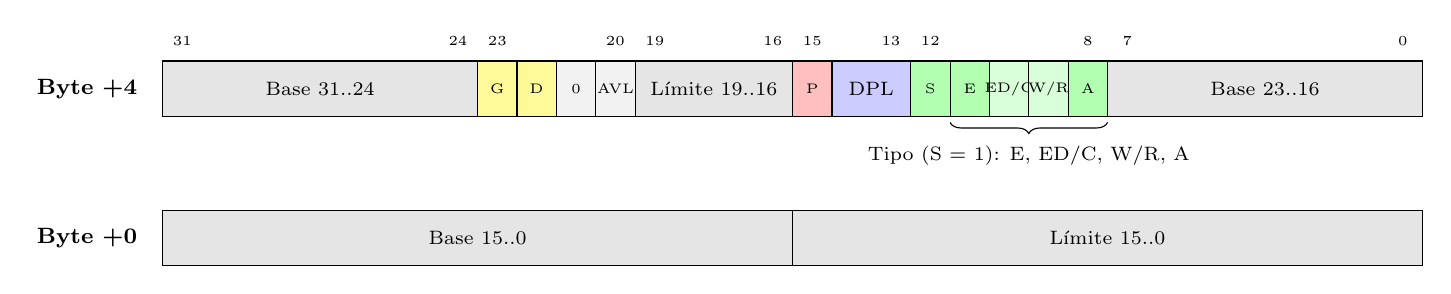
\begin{tikzpicture}[font=\scriptsize]
    \shorthandoff{<>}
    \newcommand{\bitcell}[5]{% y, high bit, low bit, texto, color
        \pgfmathsetmacro{\xa}{(31-#2)*0.5}\pgfmathsetmacro{\xb}{(32-#3)*0.5}%
        \draw[fill=#5] (\xa,#1) rectangle (\xb,{#1-0.7});%
        \node[align=center] at ({(\xa+\xb)/2},{#1-0.35}) {#4};}
    % cabecera de bits
    \foreach \b in {31,24,23,20,19,16,15,13,12,8,7,0} {
        \node[font=\tiny] at ({(31-\b+0.5)*0.5},0.25) {\b};}
    \node[anchor=east, font=\footnotesize\bfseries] at (-0.2,-0.35) {Byte +4};
    \node[anchor=east, font=\footnotesize\bfseries] at (-0.2,-2.25) {Byte +0};
    % dword alto (bits 63..32)
    \bitcell{0}{31}{24}{Base 31..24}{gray!20}
    \bitcell{0}{23}{23}{\tiny G}{yellow!40}
    \bitcell{0}{22}{22}{\tiny D}{yellow!40}
    \bitcell{0}{21}{21}{\tiny 0}{gray!10}
    \bitcell{0}{20}{20}{\tiny AVL}{gray!10}
    \bitcell{0}{19}{16}{Límite 19..16}{gray!20}
    \bitcell{0}{15}{15}{\tiny P}{red!25}
    \bitcell{0}{14}{13}{DPL}{blue!20}
    \bitcell{0}{12}{12}{\tiny S}{green!30}
    \bitcell{0}{11}{11}{\tiny E}{green!30}
    \bitcell{0}{10}{10}{\tiny ED/C}{green!15}
    \bitcell{0}{9}{9}{\tiny W/R}{green!15}
    \bitcell{0}{8}{8}{\tiny A}{green!30}
    \bitcell{0}{7}{0}{Base 23..16}{gray!20}
    % dword bajo
    \bitcell{-1.9}{31}{16}{Base 15..0}{gray!20}
    \bitcell{-1.9}{15}{0}{Límite 15..0}{gray!20}
    % llaves
    \draw[decorate, decoration={brace, mirror, amplitude=4pt}] ({(31-11)*0.5},-0.78) -- ({(32-8)*0.5},-0.78) node[midway, below=5pt] {\scriptsize Tipo (S = 1): E, ED/C, W/R, A};
\end{tikzpicture}}
\caption{Formato del descriptor de segmento de 8 bytes (S = 1) y ubicación de los bits G, D, P, S, E, A.}
\label{fig:descriptor}
\end{figure}

\begin{itemize}
    \item \textbf{GDTL (Global Descriptor Table Limit):} Campo de 16 bits del registro GDTR que indica el tamaño límite de la GDT, expresado en \emph{bytes} (offset del último byte válido). La cantidad de descriptores es \((\mathrm{GDTL}+1)/8\); con el máximo de \texttt{FFFFh} caben 8192 descriptores.
    \item \textbf{GDTR (Global Descriptor Table Register):} Registro de 48 bits que almacena la dirección base lineal (32 bits) y el límite (16 bits) de la GDT en memoria RAM. Se carga con la instrucción \texttt{LGDT}.
    \item \textbf{RPL (Requested Privilege Level):} Bits 0-1 del selector. Indica el nivel de privilegio que el programa \textit{solicita} para acceder al segmento.
    \item \textbf{LDTR (Local Descriptor Table Register):} Registro que almacena el selector del descriptor de la LDT actual (ubicado en la GDT) y mantiene una caché oculta con la base y el límite de la LDT de la tarea en ejecución. Se carga con \texttt{LLDT}.
    \item \textbf{Bit G (Granularity):} Si es 0, el límite se interpreta en bytes (máximo 1 MB). Si es 1, el límite se interpreta en páginas de 4 KB (multiplicado por 4096, máximo 4 GB).
    \item \textbf{Bit D (Default Operation Size):} Si es 0, el segmento de código opera por defecto en 16 bits. Si es 1, opera en 32 bits (afecta a operandos y direcciones). En segmentos de pila este bit se llama B y define si se usa SP o ESP.
    \item \textbf{Bit P (Present):} Indica si el segmento está cargado en memoria física. Si es 0, cualquier acceso genera una excepción de ``Segment Not Present'' (\#NP).
    \item \textbf{Bit S (System):} Si es 0, el descriptor es de Sistema (TSS, LDT, compuertas). Si es 1, el descriptor es de Código o Datos.
    \item \textbf{Bit E (Executable):} Bit 3 del campo Tipo (válido con S = 1). Si es 1, el segmento es de Código (ejecutable). Si es 0, es de Datos.
    \item \textbf{Bit A (Accessed):} El procesador lo pone en 1 automáticamente cuando el selector del segmento es cargado en un registro de segmento. El SO lo usa para saber qué segmentos han sido utilizados y cuáles pueden ser liberados.
\end{itemize}

\subsection*{d. Práctica: Diagrama interpretando el selector CS = A3FF}
Dado el selector \texttt{A3FF} en hexadecimal, lo convertimos a binario para analizar sus campos:
\texttt{A3FF = 1010 0011 1111 1111}

\begin{figure}[H]
\centering
\resizebox{\textwidth}{!}{%
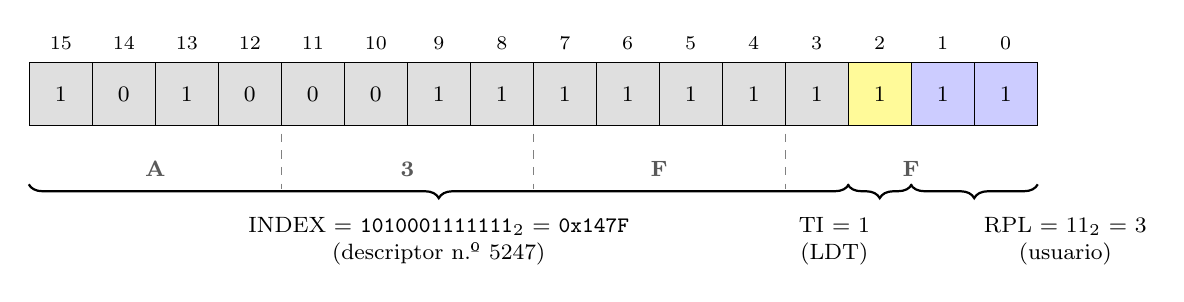
\begin{tikzpicture}[font=\footnotesize,
    bit/.style={draw, rectangle, minimum width=0.8cm, minimum height=0.8cm, align=center, inner sep=0pt}]
    \shorthandoff{<>}
    % bits (15 ... 0)
    \foreach \i/\v/\c in {15/1/gray!25, 14/0/gray!25, 13/1/gray!25, 12/0/gray!25, 11/0/gray!25, 10/0/gray!25, 9/1/gray!25, 8/1/gray!25, 7/1/gray!25, 6/1/gray!25, 5/1/gray!25, 4/1/gray!25, 3/1/gray!25, 2/1/yellow!40, 1/1/blue!20, 0/1/blue!20} {
        \node[bit, fill=\c] (b\i) at ({(15-\i)*0.8},0) {\v};
        \node[font=\scriptsize] at ({(15-\i)*0.8},0.65) {\i};
    }
    % nibbles hexadecimales
    \foreach \n/\h in {15/A, 11/3, 7/F, 3/F} {
        \node[font=\footnotesize\bfseries, text=gray!70!black] at ({(15-\n+1.5)*0.8},-0.95) {\h};
    }
    \draw[gray, dashed] (2.8,-0.5) -- (2.8,-1.2);
    \draw[gray, dashed] (6.0,-0.5) -- (6.0,-1.2);
    \draw[gray, dashed] (9.2,-0.5) -- (9.2,-1.2);

    % llaves
    \draw[decorate, decoration={brace, mirror, amplitude=5pt}, thick] ([yshift=-1.55cm]b15.north west) -- ([yshift=-1.55cm]b3.north east) coordinate[midway] (mi);
    \draw[decorate, decoration={brace, mirror, amplitude=5pt}, thick] ([yshift=-1.55cm]b2.north west) -- ([yshift=-1.55cm]b2.north east) coordinate[midway] (mt);
    \draw[decorate, decoration={brace, mirror, amplitude=5pt}, thick] ([yshift=-1.55cm]b1.north west) -- ([yshift=-1.55cm]b0.north east) coordinate[midway] (mr);
    \node[anchor=north, align=center] at ([yshift=-0.3cm]mi) {INDEX = \texttt{1010001111111}$_2$ = \texttt{0x147F}\\ (descriptor n.º 5247)};
    \node[anchor=north east, align=center] at ([yshift=-0.3cm]mt) {TI = 1\\ (LDT)};
    \node[anchor=north west, align=center] at ([yshift=-0.3cm]mr) {RPL = 11$_2$ = 3\\ (usuario)};
\end{tikzpicture}}
\caption{Interpretación del Selector CS = A3FF.}
\label{fig:selector}
\end{figure}

\textbf{Interpretación:}
\begin{itemize}
    \item \textbf{Index = 0x147F (5247):} El procesador buscará el descriptor número 0x147F en la tabla indicada. Su posición dentro de la tabla es \(\mathrm{INDEX}\times 8 = \texttt{0xA3F8}\) bytes a partir de la base de la tabla; para que el acceso sea válido, el límite de esa tabla debe ser al menos \texttt{0xA3FF}.
    \item \textbf{TI = 1:} El bit TI está en 1, por lo tanto, el índice apunta a la \textbf{LDT} (Local Descriptor Table), cuya base y límite están en el LDTR.
    \item \textbf{RPL = 3:} El nivel de privilegio solicitado es 3 (el más bajo, típico de modo usuario). Como el selector está en CS, su RPL es además el CPL actual: el código se ejecuta con privilegio de usuario, y el descriptor de código elegido debe tener DPL = 3.
\end{itemize}

% ============================================================
\section{Descriptores de Segmento y Descriptores de Sistema}
% ============================================================

\subsection*{a. Tablas de descriptores en la arquitectura 80x386}
En la arquitectura IA-32 (80x386), existen \textbf{3 tablas de descriptores} principales:

\begin{enumerate}
    \item \textbf{GDT (Global Descriptor Table):} Es la tabla principal del sistema. Contiene descriptores de segmentos de código, datos y sistema que son compartidos por todas las tareas (código del kernel, datos globales, descriptores de LDT, TSS, etc.). Solo hay una GDT por sistema, y su primer descriptor (índice 0) es nulo.
    \item \textbf{LDT (Local Descriptor Table):} Es una tabla opcional por cada tarea. Contiene descriptores de los segmentos exclusivos de esa tarea (código de la aplicación, datos locales, pila). Cada LDT está definida por un descriptor de sistema dentro de la GDT.
    \item \textbf{IDT (Interrupt Descriptor Table):} Es la tabla de descriptores de interrupciones. Contiene hasta 256 entradas (puertas de interrupción, de trap o de tarea) que mapean los tipos de interrupción y excepciones a sus correspondientes rutinas de atención (handlers). Su ubicación la da el registro IDTR.
\end{enumerate}

\textit{Nota: No debe confundirse ``tabla de descriptores'' (las estructuras GDT, LDT, IDT) con ``descriptor'' (la estructura de 8 bytes que describe un segmento o una compuerta).}

\subsection*{b. El bit S como atributo del descriptor}
El bit S (bit 12 del segundo dword del descriptor, ver Figura~\ref{fig:descriptor}) define qué clase de objeto describe la entrada, y por lo tanto cómo se interpretan los 4 bits del campo Tipo:
\begin{itemize}
    \item \textbf{S = 1:} el descriptor es un \textbf{descriptor de segmento} (de código o de datos). El campo Tipo contiene los bits E (ejecutable), ED/C (expand-down para datos, conforming para código), W/R (escribible para datos, legible para código) y A (accedido).
    \item \textbf{S = 0:} el descriptor es un \textbf{descriptor de sistema}. El campo Tipo selecciona qué objeto de sistema se describe.
\end{itemize}

\begin{table}[H]
\centering
\small
\begin{tabular}{@{}cll@{}}
\toprule
\textbf{Tipo} & \textbf{Descriptor de sistema (S = 0)} & \textbf{Dónde puede estar} \\
\midrule
\texttt{1h} / \texttt{3h} & TSS de 16 bits (disponible / ocupado) & GDT \\
\texttt{2h} & LDT & GDT \\
\texttt{4h} & Call Gate de 16 bits & GDT, LDT \\
\texttt{5h} & Task Gate & GDT, LDT, IDT \\
\texttt{6h} / \texttt{7h} & Interrupt / Trap Gate de 16 bits & IDT \\
\texttt{9h} / \texttt{Bh} & TSS de 32 bits (disponible / ocupado) & GDT \\
\texttt{Ch} & Call Gate de 32 bits & GDT, LDT \\
\texttt{Eh} / \texttt{Fh} & Interrupt / Trap Gate de 32 bits & IDT \\
\bottomrule
\end{tabular}
\caption{Tipos de descriptores de sistema del 80x386.}
\end{table}

Además, con S = 1 existen dos tipos de descriptores de segmento: \textbf{datos} (E = 0) y \textbf{código} (E = 1).

\subsection*{c. ``Call via Gate''}
Un \textbf{Call Gate} (compuerta de llamada) es un descriptor de sistema (tipo \texttt{Ch} en 32 bits) que permite que un programa de menor privilegio llame, de forma \emph{controlada}, a código de mayor privilegio. En lugar de apuntar directamente al segmento de código destino (lo cual la protección impediría si el DPL es menor al CPL), el programa ejecuta un \texttt{CALL FAR selector:offset} donde el \textbf{selector apunta al Call Gate} y el offset de la instrucción es ignorado.

\begin{figure}[H]
\centering
\resizebox{\textwidth}{!}{%
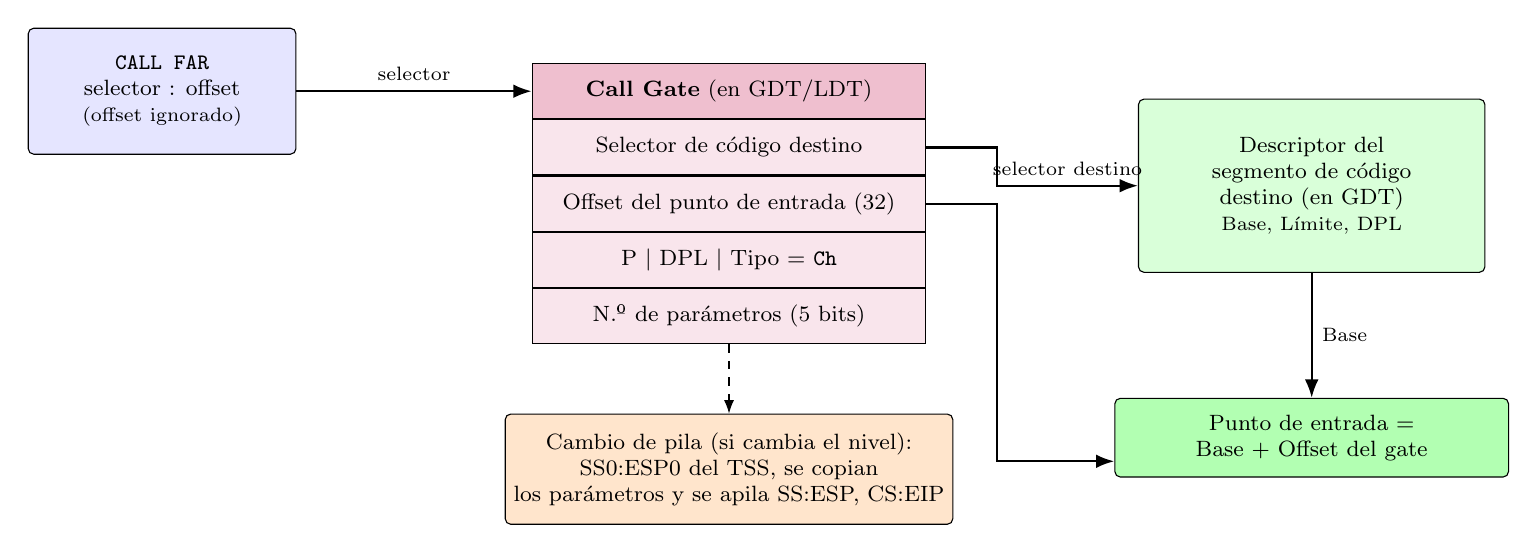
\begin{tikzpicture}[font=\footnotesize,
    blk/.style={draw, align=center, minimum height=7mm, inner sep=2pt},
    gate/.style={blk, minimum width=50mm, fill=purple!10},
    big/.style={draw, rounded corners=2pt, align=center, inner sep=3pt}]
    \shorthandoff{<>}
    \node[big, fill=blue!10, minimum width=34mm, minimum height=16mm] (call) at (0,3.6) {\texttt{CALL FAR}\\ selector : offset\\ {\scriptsize (offset ignorado)}};

    \node[gate, fill=purple!25] (gh) at (7.2,3.6) {\textbf{Call Gate} (en GDT/LDT)};
    \node[gate, below=0pt of gh] (g1) {Selector de código destino};
    \node[gate, below=0pt of g1] (g2) {Offset del punto de entrada (32)};
    \node[gate, below=0pt of g2] (g3) {P $|$ DPL $|$ Tipo = \texttt{Ch}};
    \node[gate, below=0pt of g3] (g4) {N.º de parámetros (5 bits)};

    \node[big, fill=green!15, minimum width=44mm, minimum height=22mm] (code) at (14.6,2.4) {Descriptor del\\segmento de código\\destino (en GDT)\\ {\scriptsize Base, Límite, DPL}};

    \node[big, fill=green!30, minimum width=50mm, minimum height=10mm] (entry) at (14.6,-0.8) {Punto de entrada =\\ Base + Offset del gate};

    \node[big, fill=orange!20, minimum width=44mm, minimum height=14mm] (stk) at (7.2,-1.2) {Cambio de pila (si cambia el nivel):\\ SS0:ESP0 del TSS, se copian\\ los parámetros y se apila SS:ESP, CS:EIP};

    \draw[-{Latex}, thick] (call.east) -- (gh.west) node[midway, above, font=\scriptsize] {selector};
    \draw[-{Latex}, thick] (g1.east) -- ++(0.9,0) |- (code.west) node[pos=.75, above, font=\scriptsize] {selector destino};
    \draw[-{Latex}, thick] (g2.east) -- ++(0.9,0) |- ([yshift=-3mm]entry.west);
    \draw[-{Latex}, thick] (code.south) -- (entry.north) node[midway, right, font=\scriptsize] {Base};
    \draw[-{Latex}, dashed] (g4.south) -- (stk.north);
\end{tikzpicture}}
\caption{Funcionamiento de un Call via Gate.}
\label{fig:callgate}
\end{figure}

\textbf{Funcionamiento:}
\begin{enumerate}
    \item La instrucción \texttt{CALL FAR} carga un selector que apunta a un descriptor de Call Gate en la GDT o LDT.
    \item El procesador verifica que el gate esté presente y que \(\max(\mathrm{CPL},\mathrm{RPL})\leq \mathrm{DPL}_{gate}\), es decir, que el llamador tenga privilegio suficiente \emph{para usar la compuerta}.
    \item Toma del gate el selector del segmento de código destino y verifica que su \(\mathrm{DPL}\leq\mathrm{CPL}\) (solo se puede transferir a igual o mayor privilegio).
    \item El punto de entrada es el \textbf{offset almacenado en el gate} (no el de la instrucción), por lo que el llamador solo puede entrar por las direcciones que el sistema operativo decidió exponer.
    \item Si cambia el nivel de privilegio, el procesador toma la nueva pila (SS0:ESP0, SS1:ESP1 o SS2:ESP2) del TSS, copia desde la pila anterior la cantidad de parámetros indicada en el gate y guarda SS:ESP y CS:EIP anteriores. Un \texttt{RET FAR} deshace el proceso.
\end{enumerate}
Así, las aplicaciones de usuario pueden invocar servicios del kernel sin poder saltar a cualquier dirección del código privilegiado.

% ============================================================
\section{Segmento de Estado de la Tarea (TSS)}
% ============================================================

\subsection*{a. Uso del TSS en la conmutación de tareas}
El \textbf{TSS} (Task State Segment) es una estructura de datos en memoria utilizada por el procesador para almacenar el \textbf{contexto de ejecución} de una tarea, es decir, el valor de los registros internos del procesador al momento de suspenderla.
Su propósito principal es permitir la \textbf{conmutación de tareas por hardware} (hardware multitasking). Cuando el procesador cambia de una tarea a otra, guarda automáticamente el estado de todos los registros del procesador (EIP, EFLAGS, registros de propósito general, registros de segmento, etc.) en el TSS de la tarea saliente, y luego carga el estado desde el TSS de la tarea entrante. Esto permite que el sistema operativo (a través de su scheduler) implemente multitarea de forma rápida y segura sin tener que guardar manualmente cada registro en la pila. Además, el TSS aporta las pilas de los niveles de privilegio 0, 1 y 2 que se usan cuando una tarea transfiere el control a un nivel más privilegiado.

\subsection*{b. Funcionamiento y esquema del TSS}
Cada TSS requiere un \textbf{descriptor de TSS} en la GDT (S = 0, tipo \texttt{9h} si está disponible o \texttt{Bh} si está ocupado, bit B = Busy). El registro de tarea (TR) contiene el selector hacia dicho descriptor y mantiene una caché oculta con la base y el límite del TSS. El \textbf{límite mínimo} es \textbf{67h}, es decir que el tamaño mínimo del TSS es de \textbf{68h = 104 bytes}; si el límite es menor se genera la excepción \#TS (tipo 0Ah). Si se usa el mapa de permisos de E/S, el TSS es más grande.

La conmutación se dispara con un \texttt{CALL} o \texttt{JMP} a un selector de TSS (o de Task Gate), con una interrupción o excepción manejada por una tarea, o con \texttt{IRET} si el flag NT (bit 14 de EFLAGS) es 1.

\newcounter{tssrow}
\newcommand{\tssy}[1]{\pgfmathsetmacro{\yt}{-#1*0.35}\pgfmathsetmacro{\yb}{-(#1+1)*0.35}\pgfmathsetmacro{\ym}{(\yt+\yb)/2}}
% fila completa: offset, texto, color
\newcommand{\tssfull}[3]{\tssy{\thetssrow}%
  \draw[fill=#3] (0,\yt) rectangle (8,\yb);\node at (4,\ym) {#2};%
  \node[anchor=east, font=\scriptsize] at (-0.15,\ym) {#1};\stepcounter{tssrow}}
% fila con campo en los 16 bits bajos y reservado arriba
\newcommand{\tsslow}[3]{\tssy{\thetssrow}%
  \draw[fill=gray!25] (0,\yt) rectangle (4,\yb);\node[font=\scriptsize,text=gray!60!black] at (2,\ym) {Reservado};%
  \draw[fill=#3] (4,\yt) rectangle (8,\yb);\node at (6,\ym) {#2};%
  \node[anchor=east, font=\scriptsize] at (-0.15,\ym) {#1};\stepcounter{tssrow}}

\begin{figure}[H]
\centering
\begin{tikzpicture}[font=\scriptsize]
    \shorthandoff{<>}
    \setcounter{tssrow}{0}
    % cabecera de bits
    \node[anchor=south west, font=\scriptsize] at (0,0.05) {31};
    \node[anchor=south, font=\scriptsize] at (4,0.05) {16\,$|$\,15};
    \node[anchor=south east, font=\scriptsize] at (8,0.05) {0};
    \node[anchor=east, font=\scriptsize\bfseries] at (-0.15,0.3) {Offset dec (hex)};
    % fila 100: I/O map base | reservado | T
    \tssy{0}
    \draw[fill=red!20] (0,\yt) rectangle (4,\yb);\node at (2,\ym) {I/O Map Base Address};
    \draw[fill=gray!25] (4,\yt) rectangle (7.7,\yb);\node[font=\scriptsize,text=gray!60!black] at (5.85,\ym) {Reservado};
    \draw[fill=yellow!40] (7.7,\yt) rectangle (8,\yb);\node[font=\scriptsize] at (7.85,\ym) {T};
    \node[anchor=east, font=\scriptsize] at (-0.15,\ym) {100 (64h)};
    \stepcounter{tssrow}
    \tsslow{96 (60h)}{LDT Segment Selector}{pink!40}
    \tsslow{92 (5Ch)}{GS}{green!20}
    \tsslow{88 (58h)}{FS}{green!20}
    \tsslow{84 (54h)}{DS}{green!20}
    \tsslow{80 (50h)}{SS}{green!20}
    \tsslow{76 (4Ch)}{CS}{green!20}
    \tsslow{72 (48h)}{ES}{green!20}
    \tssfull{68 (44h)}{EDI}{blue!12}
    \tssfull{64 (40h)}{ESI}{blue!12}
    \tssfull{60 (3Ch)}{EBP}{blue!12}
    \tssfull{56 (38h)}{ESP}{blue!12}
    \tssfull{52 (34h)}{EBX}{blue!12}
    \tssfull{48 (30h)}{EDX}{blue!12}
    \tssfull{44 (2Ch)}{ECX}{blue!12}
    \tssfull{40 (28h)}{EAX}{blue!12}
    \tssfull{36 (24h)}{EFLAGS}{red!12}
    \tssfull{32 (20h)}{EIP}{red!12}
    \tssfull{28 (1Ch)}{CR3 (PDBR)}{purple!15}
    \tsslow{24 (18h)}{SS2}{orange!25}
    \tssfull{20 (14h)}{ESP2}{orange!25}
    \tsslow{16 (10h)}{SS1}{orange!25}
    \tssfull{12 (0Ch)}{ESP1}{orange!25}
    \tsslow{8 (08h)}{SS0}{orange!25}
    \tssfull{4 (04h)}{ESP0}{orange!25}
    \tsslow{0 (00h)}{Previous Task Link}{yellow!30}
    % llaves de agrupación (de arriba hacia abajo)
    \draw[decorate, decoration={brace, amplitude=4pt}] (8.2,{-2*0.35}) -- (8.2,{-8*0.35}) node[midway, right=6pt, align=left, font=\scriptsize] {Registros de\\segmento};
    \draw[decorate, decoration={brace, amplitude=4pt}] (8.2,{-8*0.35}) -- (8.2,{-16*0.35}) node[midway, right=6pt, align=left, font=\scriptsize] {Registros de\\propósito general};
    \draw[decorate, decoration={brace, amplitude=4pt}] (8.2,{-19*0.35}) -- (8.2,{-25*0.35}) node[midway, right=6pt, align=left, font=\scriptsize] {Punteros a las pilas\\de niveles 2, 1 y 0};
\end{tikzpicture}
\caption{Esquema del Task State Segment (TSS) de 32 bits (tamaño mínimo 104 bytes). Los offsets se muestran en decimal y hexadecimal.}
\label{fig:tss}
\end{figure}

\textbf{Campos clave:}
\begin{itemize}
    \item \textbf{Previous Task Link:} Almacena el selector del TSS de la tarea anterior (usado para tareas anidadas). Junto con el flag NT de EFLAGS permite que un \texttt{IRET} vuelva a la tarea previa.
    \item \textbf{SS0, ESP0, SS1, ESP1, SS2, ESP2:} Punteros a las pilas de los niveles de privilegio 0, 1 y 2. Cuando una tarea pasa a un nivel más privilegiado (ej: de CPL=3 a CPL=0), el procesador carga automáticamente la pila desde aquí. La pila de nivel 3 se encuentra en los registros SS:ESP.
    \item \textbf{CR3:} Dirección base del Directorio de Tablas de Páginas de la tarea.
    \item \textbf{EIP, EFLAGS, Registros de Propósito General y de Segmento:} Estado de la CPU.
    \item \textbf{LDT Segment Selector:} Selector de la LDT de la tarea.
    \item \textbf{T:} Si es 1, genera una excepción de Debug cada vez que se conmuta a esta tarea.
    \item \textbf{I/O Map Base Address:} Desplazamiento de 16 bits desde el inicio del TSS hasta el mapa de bits de permisos de E/S (para permitir o denegar acceso a puertos cuando CPL $>$ IOPL).
\end{itemize}
Cuando una tarea se despacha con \texttt{CALL} o una interrupción, el procesador anota el TR actual en el \emph{Previous Task Link} y activa NT; el bit Busy del descriptor de la tarea previa permanece en 1 para evitar la reentrancia (un nuevo \texttt{CALL} a una tarea ocupada produce \#GP).

% ============================================================
\section{Paginado}
% ============================================================

\subsection*{a. Concepto de paginado y relación con el segmentado}
El \textbf{paginado} es un mecanismo de gestión de memoria que divide el espacio de direcciones lineales en bloques de tamaño fijo llamados \textbf{páginas} (generalmente de 4 KBytes). 
Su propósito principal es eliminar la fragmentación externa que produce el segmentado (cuyo tamaño es variable) y permitir la implementación de \textbf{memoria virtual}, mapeando páginas virtuales a marcos de página físicos no contiguos (y pudiendo llevar páginas poco usadas a disco).

\textbf{Relación con el segmentado:}
En el 80x386, la segmentación y el paginado son mecanismos complementarios que actúan en serie.
\begin{enumerate}
    \item La \textbf{Unidad de Segmentación} recibe la dirección lógica (Selector + Offset) y la traduce a una \textbf{dirección lineal} de 32 bits.
    \item Si el paginado está desactivado (bit PG del CR0 = 0), la dirección lineal es igual a la dirección física.
    \item Si el paginado está activado (bit PG = 1), la \textbf{Unidad de Paginación} toma la dirección lineal y la traduce a la \textbf{dirección física}.
\end{enumerate}

\subsection*{b. Funcionamiento de la Unidad de Paginación}
La unidad de paginación (parte de la MMU) traduce direcciones lineales de 32 bits a direcciones físicas utilizando un esquema de \textbf{paginación de dos niveles}:

\begin{enumerate}
    \item La dirección lineal de 32 bits se divide en tres campos:
    \begin{itemize}
        \item \textbf{Directorio (10 bits):} Índice dentro del Directorio de Tablas de Páginas (Page Directory), de 1024 entradas.
        \item \textbf{Tabla (10 bits):} Índice dentro de la Tabla de Páginas (Page Table) seleccionada, también de 1024 entradas.
        \item \textbf{Offset (12 bits):} Desplazamiento dentro de la página física de 4 KB (\(2^{12} = 4096\)).
    \end{itemize}
    \item El registro \textbf{CR3} contiene la dirección física base del Directorio de Tablas de Páginas.
    \item Los 10 bits del Directorio seleccionan una entrada (PDE - Page Directory Entry). Esta entrada apunta a la base física de una Tabla de Páginas.
    \item Los 10 bits de la Tabla seleccionan una entrada (PTE - Page Table Entry). Esta entrada contiene la dirección base del marco de página físico (Page Frame).
    \item Los 12 bits del Offset se suman a la base física del marco de página para obtener la dirección física final.
\end{enumerate}

Cada PDE/PTE (4 bytes) incluye además bits de control, entre ellos P (presente), R/W (escritura), U/S (usuario/supervisor), A (accedido) y D (modificado). Si P = 0 o se viola un permiso, se genera la excepción \#PF (Page Fault) y la dirección que la causó queda en CR2. Para no hacer dos accesos extra a memoria en cada referencia, el procesador guarda las traducciones recientes en la \textbf{TLB} (Translation Lookaside Buffer).

\begin{figure}[H]
\centering
\resizebox{\textwidth}{!}{%
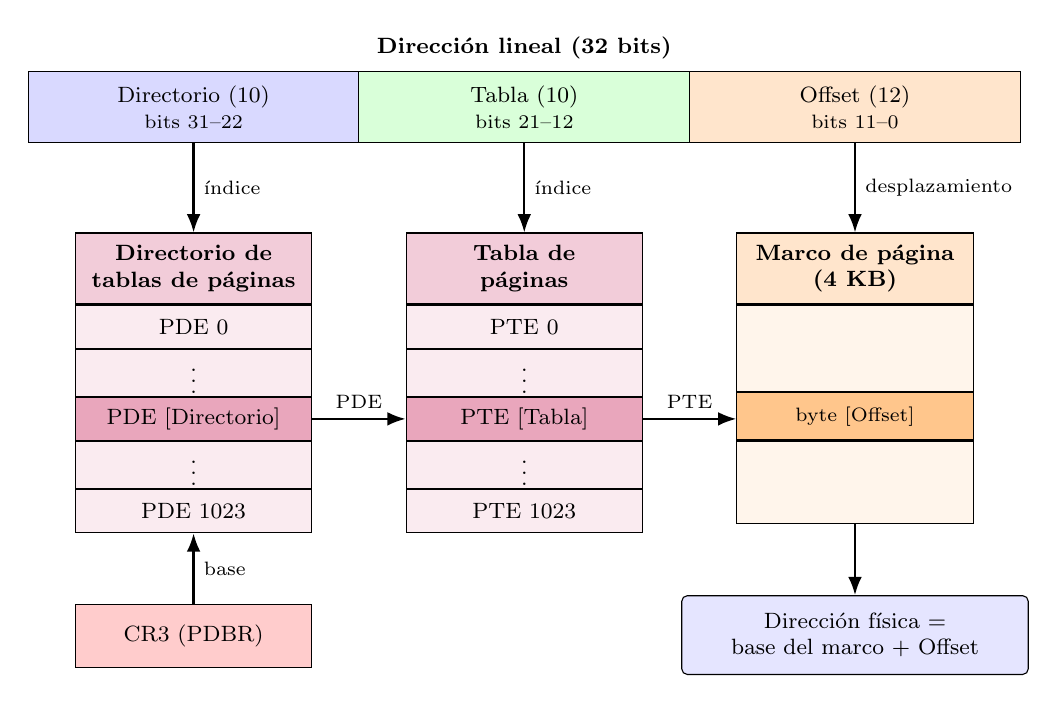
\begin{tikzpicture}[font=\footnotesize,
    fld/.style={draw, minimum height=9mm, align=center, fill=gray!20},
    trow/.style={draw, minimum width=30mm, minimum height=5.5mm, align=center, fill=purple!8, inner sep=1pt},
    thit/.style={trow, fill=purple!35},
    thead/.style={trow, fill=purple!20, font=\footnotesize\bfseries, minimum height=9mm}]
    \shorthandoff{<>}
    % dirección lineal
    \node[font=\footnotesize\bfseries] at (6.3,1.2) {Dirección lineal (32 bits)};
    \node[fld, minimum width=42mm, fill=blue!15] (fd) at (2.1,0.45) {Directorio (10)\\ {\scriptsize bits 31--22}};
    \node[fld, minimum width=42mm, fill=green!15] (ft) at (6.3,0.45) {Tabla (10)\\ {\scriptsize bits 21--12}};
    \node[fld, minimum width=42mm, fill=orange!20] (fo) at (10.5,0.45) {Offset (12)\\ {\scriptsize bits 11--0}};

    % directorio
    \node[thead] (dh) at (2.1,-1.6) {Directorio de\\tablas de páginas};
    \node[trow, below=0pt of dh] (d1) {PDE 0};
    \node[trow, below=0pt of d1] (d2) {$\vdots$};
    \node[thit, below=0pt of d2] (d3) {PDE [Directorio]};
    \node[trow, below=0pt of d3] (d4) {$\vdots$};
    \node[trow, below=0pt of d4] (d5) {PDE 1023};
    % tabla de páginas
    \node[thead] (ph) at (6.3,-1.6) {Tabla de\\páginas};
    \node[trow, below=0pt of ph] (p1) {PTE 0};
    \node[trow, below=0pt of p1] (p2) {$\vdots$};
    \node[thit, below=0pt of p2] (p3) {PTE [Tabla]};
    \node[trow, below=0pt of p3] (p4) {$\vdots$};
    \node[trow, below=0pt of p4] (p5) {PTE 1023};
    % marco de página
    \node[thead, fill=orange!20] (fh) at (10.5,-1.6) {Marco de página\\(4 KB)};
    \node[draw, minimum width=30mm, minimum height=11mm, fill=orange!8, below=0pt of fh] (f1) {};
    \node[draw, minimum width=30mm, minimum height=6mm, fill=orange!45, below=0pt of f1, font=\scriptsize] (f2) {byte [Offset]};
    \node[draw, minimum width=30mm, minimum height=10.5mm, fill=orange!8, below=0pt of f2] (f3) {};

    % CR3 y dirección física
    \node[draw, fill=red!20, minimum width=30mm, minimum height=8mm, below=9mm of d5] (cr3) {CR3 (PDBR)};
    \node[draw, fill=blue!10, rounded corners=2pt, minimum width=44mm, minimum height=10mm, align=center, below=9mm of f3] (phy) {Dirección física =\\ base del marco + Offset};

    % flechas
    \draw[-{Latex}, thick] (fd.south) -- (dh.north) node[midway, right, font=\scriptsize] {índice};
    \draw[-{Latex}, thick] (ft.south) -- (ph.north) node[midway, right, font=\scriptsize] {índice};
    \draw[-{Latex}, thick] (fo.south) -- (fh.north) node[midway, right, font=\scriptsize] {desplazamiento};
    \draw[-{Latex}, thick] (cr3.north) -- (d5.south) node[midway, right, font=\scriptsize] {base};
    \draw[-{Latex}, thick] (d3.east) -- (p3.west |- d3.east) node[midway, above, font=\scriptsize] {PDE};
    \draw[-{Latex}, thick] (p3.east) -- (f2.west |- p3.east) node[midway, above, font=\scriptsize] {PTE};
    \draw[-{Latex}, thick] (f3.south) -- (phy.north);
\end{tikzpicture}}
\caption{Esquema de traducción de paginación de dos niveles.}
\label{fig:paging}
\end{figure}

\end{document}